% !TeX program = xelatex
% Compile with XeLaTeX (Overleaf: Menu -> Compiler -> XeLaTeX)
\documentclass[12pt,a4paper]{article}

% ---------- Fonts (Carlito is metric-compatible with Calibri; free, open-license) ----------
\usepackage{fontspec}
\setmainfont{Carlito}[
  BoldFont = Carlito Bold,
  ItalicFont = Carlito Italic,
  BoldItalicFont = Carlito Bold Italic
]
% If Carlito is not available on your Overleaf install, comment the block above and
% instead uncomment the line below to fall back to a standard XeLaTeX font:
% \setmainfont{Latin Modern Sans}

% ---------- Page geometry: plain academic-paper margins ----------
\usepackage[a4paper,margin=1in]{geometry}
\usepackage{setspace}
\setstretch{1.5}

% ---------- Misc packages ----------
\usepackage{graphicx}
\usepackage{booktabs}
\usepackage{longtable}
\usepackage{array}
\usepackage[hyphens]{url}
\usepackage[hidelinks,breaklinks]{hyperref}
\usepackage{enumitem}
\usepackage{amsmath}
\usepackage{amssymb}
\usepackage[table]{xcolor}
\definecolor{coversheetgray}{HTML}{BFBFBF}

% ---------- Dotted leaders for top-level Contents entries, matching the
% List of Tables style (article.cls only dots \subsection and deeper) ----------
\makeatletter
\renewcommand{\l@section}[2]{%
  \ifnum \c@tocdepth >\z@
    \addpenalty\@secpenalty
    \addvspace{1.0em \@plus\p@}%
    \setlength\@tempdima{1.5em}%
    \begingroup
      \parindent \z@ \rightskip \@pnumwidth
      \parfillskip -\@pnumwidth
      \leavevmode \bfseries
      \advance\leftskip\@tempdima
      \hskip -\leftskip
      #1\nobreak\leaders\hbox{$\m@th\mkern \@dotsep mu\hbox{.}\mkern \@dotsep mu$}\hfill
      \nobreak\hb@xt@\@pnumwidth{\hss #2}\par
    \endgroup
  \fi}
\makeatother
\setlength{\emergencystretch}{3em}

\title{Integrating Heterogeneous Humanitarian Data for Crisis Analysis: A Source-Audit Framework Applied to Somalia}
\author{Samuel Aracena}
\date{September 2026}

\begin{document}
\raggedright

% =====================================================================
% TITLE PAGE
% =====================================================================
\begin{titlepage}
\singlespacing
\centering
\vspace*{0.6cm}
\includegraphics[width=4.5cm]{mdx_logo.jpg}
\vspace{1.2cm}

{\LARGE \bfseries INTEGRATING HETEROGENEOUS HUMANITARIAN DATA FOR CRISIS ANALYSIS: A SOURCE-AUDIT FRAMEWORK APPLIED TO SOMALIA \par}
\vspace{1.3cm}
By\par
\vspace{0.3cm}
{\large \bfseries Samuel Aracena \par}
\vspace{3cm}
A DISSERTATION\par
Submitted to\par
\vspace{0.3cm}
{\bfseries MIDDLESEX UNIVERSITY \par}
Computer Science Department\par
\vspace{0.8cm}
in partial fulfilment of the requirements\par
for the degree of\par
\vspace{0.3cm}
{\bfseries MASTER OF SCIENCE \par}
MSc Data Science\par
by Examination and Dissertation\par
\vspace{5cm}
September 2026
\end{titlepage}

% =====================================================================
% COVERSHEET (replicates the official Middlesex Dissertation/Project
% Coversheet template, layout matched cell-for-cell)
% =====================================================================
\thispagestyle{empty}
\begingroup
\singlespacing

\noindent
\begin{minipage}[b]{0.58\textwidth}
{\fontsize{16}{19}\selectfont\bfseries Middlesex University\\Computer Science Department}
\end{minipage}%
\hfill
\begin{minipage}[b]{0.35\textwidth}
\raggedleft\includegraphics[width=3.3cm]{mdx_logo.jpg}
\end{minipage}

\vspace{4pt}
\noindent\rule{\linewidth}{0.8pt}

\vspace{6pt}
\noindent{\fontsize{20}{24}\selectfont\bfseries Dissertation/Project Coversheet}

\vspace{4pt}
\noindent\rule{\linewidth}{0.8pt}
\vspace{10pt}

\begingroup
\renewcommand{\arraystretch}{1.15}
\setlength{\tabcolsep}{3pt}
\noindent\begin{tabular}{|p{4.3cm}|*{9}{p{1.04cm}|}}
\hline
\textbf{Student ID Number:} & M & 0 & 1 & 0 & 7 & 8 & 3 & 5 & 8 \\
\hline
\textbf{Student Name} & \multicolumn{9}{p{10.76cm}|}{Samuel Felipe Aracena Vicente} \\
\hline
\textbf{Module Code:} & \multicolumn{9}{p{10.76cm}|}{CST4990} \\
\hline
\textbf{Programme of Study:} & \multicolumn{9}{p{10.76cm}|}{MSc Data Science} \\
\hline
\textbf{Supervisor:} & \multicolumn{9}{p{10.76cm}|}{Giovanni Quattrone} \\
\hline
\textbf{Title:} & \multicolumn{9}{p{10.76cm}|}{Integrating Heterogeneous Humanitarian Data for Crisis Analysis: A Source-Audit Framework Applied to Somalia} \\
\hline
\textbf{Declared Word Count:} & \multicolumn{9}{p{10.76cm}|}{8739} \\
\hline
\end{tabular}
\endgroup

\vspace{10pt}
\noindent\rule{\linewidth}{0.8pt}

\vspace{6pt}
\noindent Please Note:

\vspace{4pt}
\noindent Your declared word count must be accurate, and should not mislead. Making a fraudulent statement concerning the work submitted for assessment could be considered academic malpractice and investigated as such. If the amount of work submitted is higher than that specified by the word limit or that declared on your word count, this may be reflected in the mark awarded and noted through individual feedback given to you.

\vspace{4pt}
\noindent\small It is not acceptable to present matters of substance, which should be included in the main body of the text, in the appendices (``appendix abuse''). It is not acceptable to attempt to hide words in graphs and diagrams; only text which is strictly necessary should be included in graphs and diagrams.
\normalsize

\vspace{6pt}
\noindent\rule{\linewidth}{0.8pt}

\vspace{10pt}
\noindent\fcolorbox{black}{coversheetgray}{%
\begin{minipage}{\dimexpr\linewidth-2\fboxsep-2\fboxrule\relax}
\small By submitting the dissertation you confirm you have read and understood the Middlesex University Declaration of Academic Integrity
\end{minipage}%
}
\endgroup
\clearpage

% =====================================================================
% FRONT MATTER (roman numerals)
% =====================================================================
\section*{Abstract}
\addcontentsline{toc}{section}{Abstract}

Research on diverse humanitarian topics has been widely explored, often relying on the analysis of data drawn from heterogeneous sources, such as conflict-event databases, satellite observations, market-monitoring systems and humanitarian reports. This body of work, however, shares one recurring assumption. These sources are typically treated as compatible inputs to downstream models, while the process of integrating them is treated as a technical preprocessing step rather than a decision with scientific consequences of its own.

The main aim of this dissertation is to approach data integration from a different perspective. Rather than treating integration as neutral preprocessing, the focus shifts to how integration itself is a methodological problem, one that can potentially affect the conclusions a study reaches. To study this, four data sources, ACLED (conflict), CHIRPS and VHI (climate), WFP (markets) and ReliefWeb (humanitarian reporting), are combined into one Admin-2 by month dataset for Somalia in 2024. Auditing how these sources were built and integrated, rather than assuming they are directly comparable, is the main methodological contribution of this dissertation.

Building this new dataset revealed integration challenges. An early test found districts with market data had significantly more conflict than districts without, but this did not hold up under closer inspection. Another statistical model showed ReliefWeb reporting increasing as conflict increased, as a one-standard-deviation rise in conflict translated into roughly 69\% more reports, while vegetation stress showed no major reaction in report count. A deeper analysis also checked whether some districts are just consistently more visible than others, regardless of the actual events happening on the ground. Once this is factored in, much of the conflict-tracking pattern reflects that lasting visibility rather than districts truly reacting to conflict each month. Additionally, 27 district-months across 18 districts were identified as having extreme recorded conflict or vegetation stress, but neither a WFP market observation nor a detected ReliefWeb district mention, illustrating an observability gap that this dissertation studies. Geoparser validation gives around 80\% precision but only 17.1\% pair-level recall, so these are treated as candidate gaps rather than confirmed absences of reporting.

These findings suggest that combining humanitarian data sources is a serious methodological step in its own right, with consequences for how crisis analysis is reproduced and how prediction systems trained on this kind of data behave.

\clearpage
\section*{Declaration}
\addcontentsline{toc}{section}{Declaration}

I hereby certify that this dissertation constitutes my own product, that where the language of others is set forth, quotation marks so indicate, and that appropriate credit is given where I have used the language, ideas, expressions or writings of another.

I confirm that I have not copied material from another source nor committed plagiarism nor commissioned all or part of the work (including unacceptable proof-reading) nor fabricated, falsified or embellished data when completing the attached piece of work.

I declare that the dissertation describes original work that has not previously been presented for the award of any other degree of any institution.

\vspace{0.5cm}
\noindent Signed,\\
Samuel Aracena

\clearpage
\section*{Acknowledgements}
\addcontentsline{toc}{section}{Acknowledgements}

I would like to acknowledge the organisations that made the data used in this dissertation publicly available: the Armed Conflict Location \& Event Data Project (ACLED), the Climate Hazards Group InfraRed Precipitation with Station data (CHIRPS), the Vegetation Health Index (VHI) product, the World Food Programme (WFP) and ReliefWeb, along with GADM for the administrative boundary data used to build the common analytical grid.

I would also like to thank my supervisor, Giovanni Quattrone, for his guidance and support throughout this project.

\clearpage
\setcounter{tocdepth}{1}
\tableofcontents
\clearpage
\listoftables
\clearpage
\listoffigures
\clearpage

% =====================================================================
% MAIN BODY
% =====================================================================
\section{Introduction}

Data is the main foundation behind research and scientific contribution. From the early stages of capturing mere observations to more advanced steps such as feature engineering and Exploratory Data Analysis (EDA), data transforms into meaningful insights that can be used to draw conclusions. A very important step, often overlooked as a preprocessing phase before transitioning into deeper analysis, is the integration of different data sources. Data usually varies in terms of collection method, measurement, and spatial and temporal resolution, among other factors. These differences must be considered when integrating data, as they may have a direct influence on the scientific conclusions obtained. The main focus of this dissertation is to treat this integration step as a methodological problem worth studying in its own right, rather than a routine technical task.

A humanitarian dataset has been created, using Somalia in 2024 as a case study. Data has been collected from four source categories, represented by five datasets: ACLED (conflict), CHIRPS and VHI (climate, treated as one category since both describe environmental conditions), WFP (markets) and ReliefWeb (humanitarian reporting). For brevity, these are referred to as ``the four sources'' throughout this dissertation. These sources differ in format, ranging from conflict-event databases and satellite observations to market-monitoring systems and humanitarian reports. Throughout this dissertation, the challenges that arise from integrating these data sources are explored, along with the statistical findings that result from it. Traditionally, humanitarian data has been used to predict future crises; this dissertation deviates from that approach, choosing instead to focus on the data integration aspect.

\subsection{Main research question and sub-questions}

This investigation is based on the following research question:

\begin{quote}
What methodological challenges arise when integrating heterogeneous geographic humanitarian data for crisis analysis, and how can these challenges be systematically identified?
\end{quote}

This is addressed through three sub-questions:

\begin{itemize}[leftmargin=1.5cm]
\item[RQ1.] \textbf{Data integration and quality}: How do humanitarian sources differ in spatial granularity, temporal resolution, missingness, provenance and measurement uncertainty?
\item[RQ2.] \textbf{Failure modes}: Which integration choices can introduce misleading coverage estimates, invalid features or incorrect statistical conclusions?
\item[RQ3.] \textbf{Empirical consequences}: What does applying a source-aware integration framework to Somalia reveal about humanitarian observability and reporting bias?
\end{itemize}

\clearpage
\section{Literature Review}

This chapter reviews prior work relevant to this dissertation's main topics: the recognition of data integration as a methodological problem, and the specific mechanisms by which humanitarian data sources fail to observe reality evenly. It moves from general concerns about combining heterogeneous humanitarian data, through source-specific evidence of reporting bias, to the downstream consequences such gaps produce, before identifying the gap this dissertation fills.

Bell, Lycett, Marshan and Monaghan (2021) combined eight different humanitarian datasets and found that they often do not match in terms of detail and precision, and that it is often hard to know in advance which datasets will need to be combined to answer a specific question. Due to this, a lot of potential value in humanitarian data ends up unused. They argue that the promise of big data assumes different datasets can be meaningfully connected to each other, but their own work shows this isn't always true. Based on this, they suggest five areas that need more research: data governance, data reliability, the trade-off between privacy and usefulness, transparency, and how people interact with the data. This dissertation connects most closely to two of those areas, data reliability and governance, but goes a step further by actually building and testing a method to deal with them, rather than just pointing out that they matter.

Marshak, Young and Naumova (2023) make a related point specifically about humanitarian crisis data: critical information is frequently omitted, lost or distorted, not through deliberate neglect but through the practical pressures of urgency, cost and local knowledge gaps. This reframes missingness in humanitarian data as a structural, expected pattern rather than a random gap, a framing this dissertation's own source-audit framework builds on directly.

Data governance is also explored in other publications. Haak, Ubacht, Van den Homberg, Cunningham and Van de Walle (2018) argue that the humanitarian sector needs a stronger data ecosystem, referring to systems and organisations that publish and share crisis data. This would allow a better allocation of scarce resources when disaster strikes. Recognition of this need has produced some useful tools, such as the Humanitarian Data Exchange's Data Grids (Centre for Humanitarian Data, no date). This tool tracks whether a dataset exists for a crisis-affected country, across different categories such as food security and nutrition. A dataset is only marked available if it meets three criteria: it is disaggregated below the national level, provided in a format people can use, and kept up to date. If any of these three criteria are not met, it is flagged as out of date or missing altogether. This is relevant to this dissertation because it shows that a major humanitarian institution already treats data availability as measurable and traceable, rather than simply assuming the data is already fine.

Reporting bias is another aspect that has been particularly explored in conflict event data, one of this dissertation's four sources. Weidmann (2016) uses the spread of cellphone coverage as a natural experiment to illustrate this. His findings reveal that conflict datasets fail to properly capture violence in areas with poor media access. Deadly events get picked up far more reliably than non-lethal ones, meaning remoteness itself predicts what gets recorded rather than what actually occurs. What initially looked like cellphones being responsible for more violence turned out to be cellphones causing more reporting of violence that was already happening. ACLED, one of the sources used in this dissertation, acknowledges this type of bias. Miller, Kishi, Raleigh and Dowd (2022) wrote about their agenda for tackling bias in conflict datasets, ACLED included. ACLED's acknowledgement of these limitations provides further justification for examining the spatial and reporting biases within the dataset rather than treating its event records as a complete representation of conflict.

Examples of reporting bias can also be found outside humanitarian work. Hendrix (2017) describes a ``streetlight effect'' in the context of climate research on Africa. His publication argues that researchers, as well as the data systems that support them, tend to study topics that are convenient or properly funded, rather than themes that are relevant or most in need of attention. Factors such as colonial history and existing civil liberties can predict how much research attention a topic receives, almost as much as how badly it actually needs that attention. This same principle is relevant to the four sources used in this dissertation: each observes Somalia according to its own collection mechanism and operational priorities rather than according to an objective measure of severity.

The gaps exposed by reporting bias can carry consequences for how humanitarian aid is distributed. Eisensee and Str\"omberg (2007) analysed roughly 5,000 US disaster relief decisions and found that news coverage affects the likelihood of relief being granted, even after accounting for a disaster's severity. Their work indicates that an observability gap can matter beyond the dataset itself, shaping where resources are directed. This is the kind of downstream consequence this dissertation's third research question investigates.

The literature reviewed in this chapter establishes that humanitarian data integration is a recognised structural problem (RQ1's concern), that individual sources carry documented, source-specific biases that can affect integration outcomes in many ways (RQ2's concern), and that the resulting observability gaps have measurable downstream consequences for real decisions (RQ3's concern). The literature reviewed here does not identify a study that combines these four sources into one harmonised dataset, audits their differences directly against one another using a single reproducible framework, and empirically tests what those differences do to an analytical conclusion. This dissertation addresses that gap, using Somalia in 2024 as its case study.

\clearpage
\section{Methodology}

\subsection{Data sources}

This dissertation combines four data sources, each capturing a different dimension of humanitarian conditions in Somalia during 2024: conflict, climate, markets, and reporting.

\begin{itemize}[leftmargin=1.2cm]
\item \textbf{ACLED} (Armed Conflict Location and Event Data; Raleigh et al., 2010) provides a record of conflict events, including event type, location and fatalities, compiled from media and local reporting. It is the only one of the four sources that is a direct record of discrete events rather than a continuous or periodic measurement.

\item \textbf{CHIRPS} (Climate Hazards Group InfraRed Precipitation with Station data; Funk et al., 2015) and \textbf{VHI} (Vegetation Health Index; NOAA/NESDIS STAR, no date) provide satellite-derived environmental indicators: rainfall from CHIRPS and vegetation health/stress from VHI. CHIRPS supplies monthly rainfall estimates, and VHI provides a weekly measure of vegetation stress derived from satellite imagery. Data obtained from both of these sources is used as a proxy for drought conditions. Additionally, both are raster datasets cropped to Somalia's extent with a small buffer, rather than tabular records tied to specific reported events.

\item \textbf{WFP} (World Food Programme; World Food Programme, no date) provides market price data for four commodities tracked across Somali markets. Unlike the other three sources, WFP data exists only where a functioning market is being monitored, so its coverage is a direct reflection of which places have accessible markets in the first place, not just of where prices were recorded.

The four commodities tracked (wheat flour, rice, sugar and oil) are not an arbitrary selection. These overlap substantially with Somalia's Minimum Expenditure Basket (MEB) and with the standard set of essential items used by FSNAU (the Food Security and Nutrition Analysis Unit for Somalia) to track the cost of a basic livelihood. WFP's Somalia price data covers 17 commodities in total, including sorghum, maize, potatoes, and meat. Restricting this dissertation's market layer to these four represents a deliberate focus on the commodities WFP itself treats as essential to a Somali household's basic diet, rather than an incidental subset of whatever data happened to be available.

\item \textbf{ReliefWeb} (UN OCHA, no date) provides the humanitarian reporting layer: narrative reports on the crisis, tagged by theme (such as Food and Nutrition, or Protection and Human Rights) and, where possible, geoparsed to identify which districts each report discusses.
\end{itemize}

All four sources were combined with Somalia's administrative boundaries (GADM, level 2, 74 districts; GADM, 2022) to allow every source to be located on a common map. This is straightforward for ACLED, CHIRPS and VHI, whose locations match directly to GADM's boundaries or coordinates. WFP is different: its price data uses its own market and place names, which do not always match GADM's district names, whether through spelling differences or because a market name refers to a town rather than the district containing it. A crosswalk table was therefore built manually, mapping each WFP market name to its GADM district, so the data could be joined to the grid automatically rather than through error-prone case-by-case matching.

\subsection{Common analytical grid}

Before moving into aggregating data to build the final dataset, all four sources were converted from their native formats into a single common grid: 74 districts (Admin-2 level, from the GADM boundary file) by 12 months of 2024, giving 888 district-month rows in total.

Each source required a different kind of conversion to fit this grid. ACLED's conflict events, already geocoded to specific locations, were aggregated into monthly counts per district. CHIRPS and VHI, both raster datasets, were converted using zonal statistics. For each district polygon and each month, the average rainfall or vegetation value within that polygon's boundary was calculated. WFP's market prices were matched to districts using the crosswalk table described in the previous section. ReliefWeb reports were geoparsed to identify which district or districts each report mentioned, then counted per district per month.

Before this conversion, the raw CHIRPS and VHI rasters covering the wider region were cropped to Somalia's extent plus a small buffer, reducing their size substantially without losing any information relevant to this analysis, since only the zonal statistics over the 74 districts are ever computed from them. This was verified directly: the January rainfall value calculated for one district (SO\_AADAN) matched the same figure produced by an earlier, smaller-scale version of this pipeline exactly. This is a spot-check on a single district-month rather than an exhaustive comparison, so it is evidence that the cropping step behaves as intended, not a guarantee that no district or month is affected.

The result is a single table where every row represents one district in one month, and every column represents a measurement from one of the four sources, allowing them to be compared and modelled together directly.

\subsection{Source-audit framework}

Combining four sources onto one grid is only useful if each source's own reliability is understood first. This dissertation applies a source-audit framework built around three distinctions that provide a common audit framework across the four sources, although their relevance differs by source: structural versus recorded availability, observed versus forecast values, and zero versus missing.

Structural versus recorded availability distinguishes between whether data could exist for a given place and time, and whether it actually was captured. A district with no market, for instance, cannot structurally produce WFP price data; a district with a market that simply wasn't surveyed that month is a different, and more informative, kind of gap. Collapsing these two cases into one would treat a genuine absence of infrastructure the same as a missed observation, obscuring exactly the kind of unevenness this dissertation investigates.

Observed versus forecast values matters because not every number in these datasets is necessarily a direct measurement. WFP price datasets can in general contain model-generated forecasts alongside genuinely observed transactions, and treating a forecast as equivalent to an observed price would silently mix two different kinds of evidence in the same column, making it important to check which is which before integration. The audit described in Section 4.1 was conducted specifically to determine whether this applied to the four commodities used here; it did not, with all 1,676 present values recorded as observed rather than forecast.

Zero versus missing addresses a related confusion: a district with zero recorded conflict events is not the same as a district for which no conflict data exists at all, and a modelling approach that fails to keep these separate risks either inflating or deflating apparent stability.

Applying this framework to ReliefWeb required the most additional work of any source, since its reports are unstructured text rather than structured records. Each report was geoparsed to identify which district or districts it discusses, using an alias list built from three inputs: the ACLED crosswalk, GADM's VARNAME\_2 field (which records alternate place names), and manual research into local naming conventions. This alias list covers 65 of the 74 districts. Geoparser performance was validated in two stages. An initial exercise reviewed two independent random samples of 15 matched reports each (30 in total) by hand, finding 13 of 30 (43\%) genuinely about the district they matched. That first check was small, and it scored only reports the geoparser had already matched, so it could estimate precision on that sample but could say nothing about how many district mentions were missed altogether.

A second, larger validation was therefore carried out. One hundred reports from March to December 2024 were labelled by hand without reference to the geoparser's output, drawn under a stratified design that deliberately sampled both reports the geoparser matched and reports it did not, so that misses could be counted as well as false matches. Because that design over-represents matched reports relative to their frequency in the source (1,116 eligible reports, of which 519 were matched and 597 were not), the recall figures are reweighted to population proportions. Results are reported at two levels of detail: the report-district pair (did the geoparser identify this particular district in this particular report?) and the report (did it identify that the report concerns any district at all?).

\begin{table}[h!]
\centering
\begin{tabular}{lrrr}
\toprule
\textbf{Unit scored} & \textbf{Precision} & \textbf{Recall} & \textbf{F1} \\
\midrule
Report-district pair & 81.1\% & 17.1\% & 28.2\% \\
Report & 78.8\% & 57.8\% & 66.7\% \\
\bottomrule
\end{tabular}
\caption{Geoparser validation on 100 hand-labelled reports, recall reweighted to population proportions.}
\label{tab:geoparser}
\end{table}

Precision is the stronger side and is unaffected by the stratification, since it is computed only on what the geoparser flagged: roughly four in five district matches hold up under manual review at either level of detail. Recall is the weaker side, and the gap between its two levels is the informative part. The geoparser usually recognises that a report concerns at least one district (57.8\%), but frequently misses the other districts that the same report also covers (17.1\% at the pair level). The geoparser reads only a report's exported title and body text. Geographic detail held in PDF or table attachments is one plausible explanation for the missed pairs, alongside missing aliases and unusual spellings; because the attachments were never opened, their contribution cannot be separated here.

The two exercises measure different things on different samples and should not be read as an improvement from 43\% to 81\%. The second supersedes the first and is the validation used throughout this dissertation.

Low pair-level recall has a direct consequence for how the reporting variable is interpreted. A zero in \texttt{reports\_mentioning\_district\_count} means that no district mention was detected in the exported text, not that no humanitarian reporting about that district exists. This distinction is carried through Chapter 4 wherever the absence of reporting is discussed.

This is an acknowledged limitation rather than a solved problem. Attempts to improve precision further were constrained by the environment used to build this dataset: reading report attachments, which would likely improve location accuracy, was blocked by network restrictions during this project. Rather than presenting an inflated picture of accuracy, this dissertation documents the geoparser's real precision directly and carries this limitation forward explicitly into the discussion of results, revisited in Chapter 5.

\subsection{Engineered features}

Following data preprocessing and integration, a set of 19 engineered features was built that could help us capture useful information from each one. Some of the main features will be detailed below. For a complete list of all features, please refer to Appendix A.

\subsubsection{Conflict features (ACLED)}

\textbf{Conflict count and trend}: \texttt{conflict\_event\_count} refers to the number of ACLED events recorded in a district in a given month, and \texttt{fatalities} is the sum of fatalities across those events. Its trend feature is a log-difference:
\[
\text{conflict\_trend\_log}_t = \ln(1+\text{count}_t) - \ln(1+\text{count}_{t-1})
\]
where $\text{count}_t$ is the event count in the current month and $\text{count}_{t-1}$ is the count in the previous month. The ``+1'' inside the logarithm (a log1p transform) allows the formula to handle months with zero events, which a plain logarithm cannot. This log-difference form was used instead of a plain percentage change, since percentage change is undefined whenever the previous month's value is zero, a frequent occurrence in this data rather than a rare edge case. A log-difference is also used for each commodity's price trend in Section 3.4, but without the ``+1''. Prices are strictly positive, so the plain form $\ln(P_t) - \ln(P_{t-1})$ applies there; the log1p variant is needed only for conflict counts, which can be zero.

\subsubsection{Climate features (CHIRPS/VHI)}

\textbf{rainfall\_mean\_mm} = zonal mean of the CHIRPS rainfall raster over the district's polygon, for that month:
\[
\text{zonal\_mean}(D) = \frac{1}{N}\sum_{i=1}^{N} v_i
\]
where $v_i$ is the value of the $i$-th valid raster cell overlapping district $D$, and $N$ is the number of such valid cells.

\textbf{vegetation\_health\_index\_mean} = zonal mean of the VHI raster over the district's polygon, built from weekly satellite composites weighted by how much of each week falls in the given calendar month:
\[
\text{VHI}_{\text{month}} = \frac{\sum_{w \in W} \text{zonal\_mean}(D, \text{VHI}_w) \cdot d_w}{\sum_{w \in W} d_w}
\]
where $W$ is the set of satellite weeks that overlap the target month at all, $d_w$ is the number of days of week $w$ that fall within that month (out of 7), and $\text{zonal\_mean}(D,\text{VHI}_w)$ is that week's zonal mean, as defined above.

\subsubsection{Market prices features}

\textbf{Market presence} (\texttt{has\_market\_coverage}): a binary, year-round flag indicating whether WFP monitors any market in the district at all, in any month of 2024. Unlike the price and PEWI features below, it does not vary month to month within a district; it is a structural, fixed characteristic of the district itself.

\textbf{Price}: each of the four tracked commodities (wheat flour, rice, sugar, oil) has a price converted to USD, and its own log-difference trend.

\textbf{PEWI score}: The Price Early Warning Indicator (PEWI) is WFP's own name for a method more widely known as ALPS (Alert for Price Spikes). It measures how far a commodity's price sits from its own normal seasonal pattern, classifying results into one of these phases (Normal $\leq 0.25$, Stress $0.25$--$1.0$, Alert $1.0$--$2.0$, Crisis $> 2.0$). Results are given in standardised units, which allows different commodities to be compared on the same scale. This score is already calculated by WFP and values were extracted as they are. For reference, WFP's PEWI formula goes as follows:
\[
\text{PEWI}_t = \frac{P_t - \hat{P}_t}{\sigma_\varepsilon}
\]
where $P_t$ is the actual observed price for the commodity in month $t$; $\hat{P}_t$ is the estimated ``normal'' seasonal price for that same month, based on the commodity's own historical seasonal pattern (so it accounts for prices naturally rising or falling at certain times of year, rather than flagging normal seasonal variation as an anomaly); and $\sigma_\varepsilon$ is the historical standard deviation of the residuals (the gaps between actual and estimated seasonal prices), which puts the whole measure in standardised units so it's comparable across commodities with very different price levels.

\subsubsection{Reporting features}

Both features rely on the geoparsing method described in Section 3.3, which matches each report's text against a district's official name or documented alias.

\begin{itemize}
\item \texttt{reports\_mentioning\_district\_count} = COUNT of reports whose title or body text matches the district's official name or a documented alias.
\item \texttt{food\_nutrition\_report\_count} = COUNT of the above, restricted to reports whose themes field contains ``Food and Nutrition.''
\end{itemize}

\subsubsection{Standardisation for modelling}

Two variables described above, logged conflict counts and a vegetation-stress measure (the negative of the Vegetation Health Index, so that higher values consistently mean more stress for both conflict and climate), are converted to z-scores before entering the statistical models used in Chapter 4. This puts both variables on the same scale, so that a model coefficient can be read as ``the effect of a one standard deviation increase,'' making the size of the conflict association and the vegetation-stress association directly comparable. This matters because a central comparison in this dissertation is exactly this: whether reporting attention responds more strongly to conflict than to climate stress, and that comparison is only meaningful once both predictors are expressed in the same units.

\subsubsection{Features used in modelling}

Not every one of the 19 engineered features was used as a predictor, and the two model families draw on different subsets by design. The negative binomial models (Sections 4.3 and 4.4) use only conflict counts (logged and standardised) and vegetation stress (standardised), with month controls and, in the fixed-effects check, district controls: adding market, rainfall or region controls would answer a different question from the conflict-versus-vegetation-stress comparison those models isolate. The supplementary logistic regression (Section 3.5) asks the broader question of what predicts reporting coverage at all, and so draws on a wider set: conflict (logged), market presence (\texttt{has\_market\_coverage}), rainfall, vegetation stress, and region and month controls. Table~\ref{tab:modelspecs} sets out which predictors enter which model. The individual commodity prices, PEWI scores and \texttt{conflict\_trend\_log} were constructed and audited as part of this dataset and used in the missingness analysis and the WFP audit, but were not fed into either model family. \texttt{food\_nutrition\_report\_count} is used once as an alternate outcome variable, not as a predictor.

\subsection{Statistical modelling approach}

Two kinds of outcome are modelled in this dissertation, each requiring a different regression approach.

Reporting counts (how many reports mention a district in a given month) are modelled using negative binomial regression. This is appropriate for count data because a linear regression does not naturally respect the non-negative, discrete nature of counts. On the other hand, a simpler Poisson model assumes the conditional mean and variance are equal and can therefore be inappropriate when the data are overdispersed, meaning the variance in report counts is larger than a Poisson model assumes. The main model takes the form:
\[
\text{reports}_{it} = f(\text{conflict\_z}_{it},\ \text{vhi\_stress\_z}_{it},\ \text{month}_t)
\]
$\text{month}_t$ adds one indicator variable for each calendar month. This controls for anything that makes reporting go up or down nationwide in a given month for reasons that have nothing to do with conflict or climate, such as seasonal patterns or number of ReliefWeb reports published that month. With this control in place, the conflict and vegetation-stress effects reflect comparisons made within the same month, rather than a seasonal trend being mistaken for a real effect.

Standard errors are also clustered by district throughout. Each district contributes 12 monthly rows to the data, but these rows are not independent observations of 12 different places; they are the same place observed twelve times. Treating them as independent would understate how uncertain the results really are.

Rather than comparing empirically the conflict and vegetation-stress coefficients, a Wald test is used to formally test whether the two effects are statistically different in size from one another. The Wald test formally supports the claim that the estimated conflict association is statistically larger than the estimated vegetation-stress association in this pooled specification.

Banaadir (Mogadishu's region) is excluded from this main model, since it is mentioned in all 12 months of 2024 without exception, matching the sample used in the logistic regression described below, where its inclusion causes a statistical problem called perfect separation (a predictor that perfectly determines the binary outcome drives that model's coefficient towards infinity). For the negative binomial model, Banaadir's exclusion is instead checked directly by re-fitting the same specification on the full panel with Banaadir included, which confirms the headline result is not sensitive to the exclusion.

The same negative binomial formula, with the same standardisation, cluster-robust standard errors and Wald test, is reused for two further purposes: testing whether the headline pattern holds when the outcome is restricted to Food and Nutrition reports only (Section 4.3), and testing whether it survives once district fixed effects are added (Section 4.4), controlling for permanent differences between districts rather than only between months. Region is omitted there, being a time-invariant district characteristic that the fixed effects would absorb entirely. Adding fixed effects for the 73 districts in this sample (Banaadir excluded, $n = 876$) requires many more parameters, and the standard optimizer failed to converge, so the model was fit with L-BFGS. To check the result was not an artefact of that choice, the specification was re-estimated with an alternative optimizer (BFGS, started from the L-BFGS solution, since it does not converge from default starting values at this dimension) and with a different model family (Poisson/PPML, the appropriate comparison since the fitted overdispersion collapses to essentially zero once fixed effects are included). All three reach effectively the same log-likelihood and agree on the conflict coefficient to three decimal places, an incidence rate ratio of 1.024 in every case.

Whether a district is mentioned at all (a yes/no outcome, examined here as a supplementary analysis of reporting coverage) is modelled instead with logistic regression, again with cluster-robust standard errors by district. This model is validated out-of-sample using group k-fold cross-validation, which holds out entire districts rather than individual district-months, so the model is tested on places it has never seen at all, a stricter and more meaningful test of generalisation than holding out random rows would be. Performance in this out-of-sample setting is measured using AUC (area under the ROC curve), which summarises how well the model ranks districts by predicted coverage likelihood, independent of any particular probability threshold. Full diagnostics for this model, including accuracy, precision, recall, specificity and the confusion matrix, are provided in Appendix D.

The exact specification of every regression used in Chapter 4, including which predictors, fixed effects and standard-error correction produced each result, is given in Appendix E (Table~\ref{tab:modelspecs}).

\clearpage
\section{Data Analysis \& Results}

\subsection{RQ1: Data integration and quality}

RQ1 asked how humanitarian sources differ in spatial granularity, temporal resolution, missingness, provenance and measurement uncertainty. This section summarises what the source-audit framework (Chapter 3) found when applied directly to the four sources. A full source-by-source comparison across all seven dimensions is provided in Appendix B.

Spatial granularity varies sharply between sources. ACLED's conflict events are geocoded at the point level, but not uniformly precisely: 77.5\% (2,673 of 3,448) of Somalia's 2024 events are coded to an exact site, 22.4\% (772) to only an approximate location, and 0.1\% (3) to no more than the broad surrounding area. CHIRPS and VHI are raster-based rather than point-based: CHIRPS at 0.05-degree resolution and VHI at approximately 0.036-degree resolution, aggregated to the district level via zonal statistics rather than observed directly at that level. WFP prices and ReliefWeb reports are structurally different again: prices are tied to specific monitored markets, and reports are unstructured text carrying country-level metadata but no district-level location field, requiring the geoparsing step described in Section 3.3.

Provenance also differs. ACLED's events are compiled from media reports and local sourcing, a human third-party coding process, which is consistent with its spatial precision varying event by event. CHIRPS and VHI are primarily satellite-derived and algorithmically processed, though CHIRPS is not purely remote: as its full name records (Climate Hazards Group InfraRed Precipitation with Station data), it blends infrared satellite estimates with ground station observations. What both share, and what distinguishes them from ACLED, is the absence of a per-record human coding step, which largely explains why their coverage is complete rather than uneven. WFP's prices come from enumerators physically visiting markets. ReliefWeb curates humanitarian organisations' own published material, applying shared taxonomies without independently verifying each report's contents. These four origins, human coding, satellite algorithms, field surveys and organisational publication, each offer a different lens onto the same reality.

Temporal resolution also differs. ACLED and WFP prices are available at the finest grain this dissertation uses (monthly, aggregated from daily events or observations), CHIRPS is published at daily, pentadal and monthly resolutions, with the monthly product used here, and VHI is only available as weekly composites, requiring the day-weighted aggregation described in Section 3.4 to bring it onto the same monthly grid as everything else.

Missingness is structurally, not randomly, distributed. Market presence is itself a year-round, district-level fact: only 35 of 74 districts (47.3\%) have a WFP-monitored market at all. This ceiling doesn't change month to month. Across all 888 district-months, each commodity's price is missing in 469 of them (52.8\%), driven almost entirely by the 39 structurally-unmonitored districts ($39 \times 12 = 468$ district-months) rather than by gaps within the 35 monitored ones, where price coverage is close to complete. Price and PEWI availability are not identical and should not be quoted as one figure. PEWI is missing more often, in 505 district-months for wheat flour, sugar and oil and 508 for rice, because it additionally requires enough price history to compute an anomaly score; the trend features are missing in 504 for the same reason, each district's first observed month having no previous value to difference against. Across the four commodities, at least one price is present in 419 district-months (47.2\%) and at least one PEWI score in 383 (43.1\%). This pattern persisted from the two-month prototype into the full panel, indicating a structural feature of market monitoring rather than a random collection gap. The month-by-month breakdown for all four sources is in Appendix C.

As an additional analysis of reporting coverage, complementing the comparisons above rather than directly answering RQ1's question about source characteristics, a logistic regression was used to examine whether basic reporting coverage, whether a district was mentioned at all in a given month, could be predicted from conflict, market coverage, climate and regional and month controls (Section 3.5). The full model reached an in-sample AUC of 0.776, but its out-of-sample AUC, tested on districts held out entirely, fell to 0.641. Removing region and climate together, the climate terms adding almost nothing once conflict, market, region and month are in the model (chi-squared = 0.20, p = 0.91) while region improves in-sample fit substantially (chi-squared = 60.41, p < 0.0001), produced a lower in-sample AUC (0.739) but a higher out-of-sample AUC of 0.716, meaning regional information contributed to apparent in-sample fit while actually reducing how well the model generalised to districts it had not seen. Full diagnostics for both versions are in Appendix D. This is a second, independent line of evidence that district-level identity can look more informative than it really is once tested on unseen data.

Measurement uncertainty was checked directly rather than assumed. The concern was whether WFP's market data is genuinely observed or partly the organisation's own model-generated forecast presented in the same columns. Auditing the four commodities across all of 2024 found 99.8\% genuinely observed (1,676 of 1,680 possible district-commodity-month values, from 35 monitored districts across 12 months and 4 commodities), with no forecast values in any month. The four missing cells trace to a single documented collection gap (Banaadir in January), not to forecast substitution.

Taken together, these findings answer RQ1 directly. The four sources differ substantially: in how precisely they locate events, where their data actually comes from, how often they report, and how completely they cover the country. These differences are structural properties of each source, not incidental noise. That distinction is exactly the premise the rest of this dissertation's argument depends on.

\subsection{RQ2: Failure modes}

RQ2 asked which integration choices can introduce misleading coverage estimates, invalid features, or incorrect statistical conclusions. This section presents concrete cases where getting the integration wrong actually changed a result, not just cases where it hypothetically could.

Pseudo-replication produced a false positive. A Mann-Whitney U test first compared conflict-event counts between districts with and without WFP market coverage at the district-month level, treating all 888 rows as independent, and found a significant relationship ($p = 0.0001$). But market status barely changes month to month within a district, so treating those rows as independent counted each of the 74 districts roughly twelve times over. Repeating the same test on one row per district, using each district's average conflict level, gave $p = 0.18$. The apparent significance did not survive aggregation, showing the naive inference was sensitive to treating repeated district-months as independent. This does not establish that no relationship exists between markets and conflict; it establishes that the evidence for one is not robust to using the district, rather than the district-month, as the unit of analysis.

Feature engineering choices can also fail silently. An early version of this pipeline calculated trends as a percentage change from the previous month. This measure is mathematically undefined whenever the previous month's value is zero, which happens often enough in this data to be a real problem rather than a rare edge case. Left unchecked, this would have produced missing or invalid values embedded silently inside an otherwise complete-looking column. It was replaced with a log-difference formula, which handles zero values correctly.

Not every engineered feature turns out to measure what it claims to. \texttt{conflict\_density}, conflict events divided by district area, was built on the assumption that it would better represent humanitarian intensity than a plain event count. Testing this directly showed the opposite: it correlated with the plain event count at $r = 0.96$, meaning it carried almost no independent information, correlated with district area at $r = -0.34$ overall ($r = -0.64$ among conflict-affected districts only), tracking district size more closely than anything genuinely humanitarian, and predicted fatalities worse than the raw count did ($r = 0.727$ versus $0.776$ for the raw count).

Conflating a zero with a missing value is a further, more conceptual failure mode. A district with zero recorded conflict events is not the same as a district for which no conflict data exists at all. Collapsing these two cases into one, as a careless integration might, would either overstate how calm a place is or understate how much is genuinely unknown about it. The source-audit framework's structural-versus-recorded distinction (Section 3.3) exists specifically to keep this failure mode from entering the analysis undetected. Because ACLED has structural coverage across all 74 districts, an absent event record in this dataset is interpreted as zero recorded events rather than missing source coverage; it does not imply that no violence occurred.

Together these four cases answer RQ2 concretely: integration choices are not neutral bookkeeping. Each was caught only because it was tested directly rather than assumed correct, which is the audit-first approach applied throughout this dissertation.

\subsection{RQ3: Empirical consequences}

RQ3 asked what applying this source-aware integration framework to Somalia reveals about humanitarian observability and reporting bias. This is where the methodology developed in Chapter 3 is put to direct empirical use.

One of the main findings is that reporting volume is strongly associated with recorded conflict, but shows no comparable association with vegetation stress. In the main model (Section 3.5), a one standard deviation increase in logged conflict counts is associated with an incidence rate ratio of 1.69 (95\% CI [1.39, 2.06], $p < 0.0001$), so reports increase by approximately 69\% per standard deviation, holding month and vegetation stress fixed. Vegetation stress is not significantly associated with reporting volume in this pooled specification: an IRR of 0.996 (95\% CI [0.78, 1.27], $p = 0.97$), indistinguishable from no relationship. A Wald test confirms the two coefficients differ significantly in magnitude (chi-squared $= 9.15$, $p = 0.0025$). The choice of negative binomial over Poisson is supported by the fitted overdispersion parameter (alpha $= 1.330$, $p < 0.0001$), which is well above zero, so the variance in report counts exceeds what Poisson would assume.

Figure~\ref{fig:attention} shows this relationship directly, plotting expected ReliefWeb reports across the percentile range of each measure within Somalia's 2024 distribution. The conflict curve rises steeply toward the upper percentiles, while the vegetation-stress curve stays essentially flat across the entire range, a visual counterpart to the IRR estimates above.

\begin{figure}[h!]
\centering
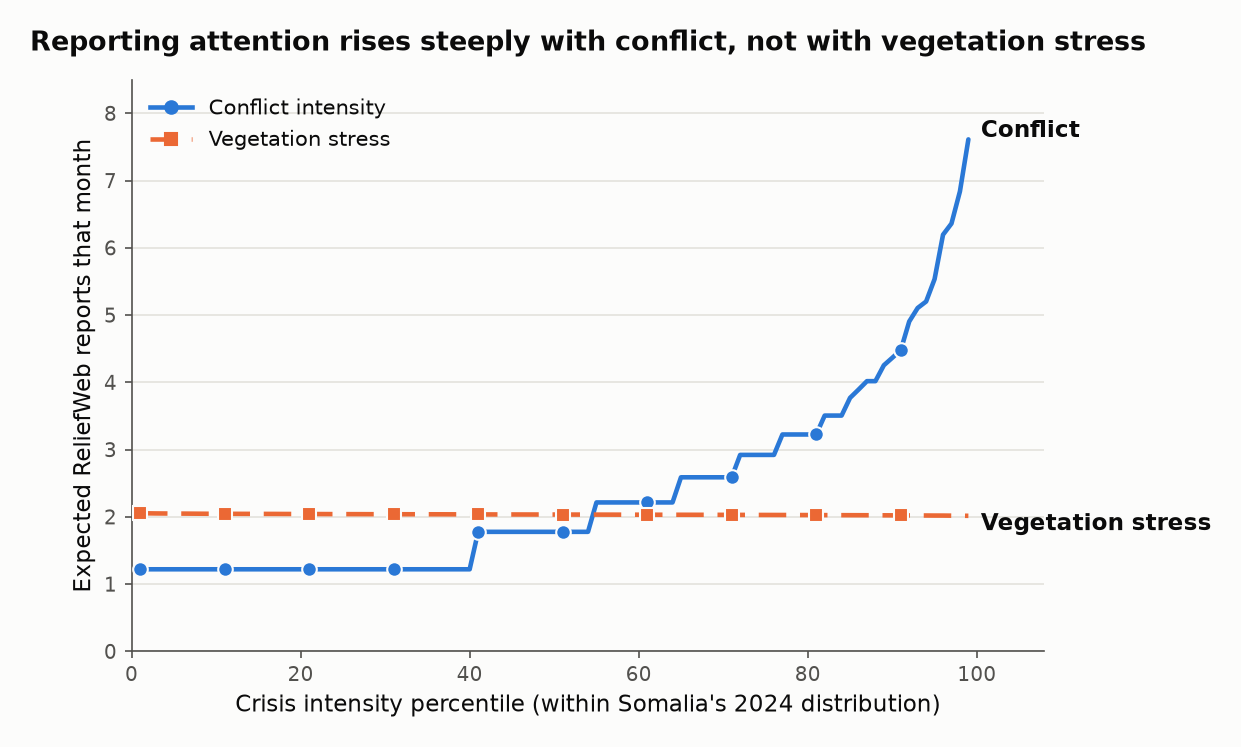
\includegraphics[width=0.85\linewidth]{attention_response_curve.png}
\caption{Expected ReliefWeb reports per district-month, by crisis-intensity percentile: conflict intensity versus vegetation stress.}
\label{fig:attention}
\end{figure}

One objection is that conflict events might simply generate more reports of any kind, inflating the overall count without reflecting attention to humanitarian need specifically. To test this, the same analysis was repeated with the outcome restricted to reports ReliefWeb itself tags ``Food and Nutrition''. The pattern persists: conflict corresponds to a significant increase in reporting count (IRR $= 1.78$, 95\% CI [1.46, 2.18], $p < 0.0001$), vegetation stress remains non-significant (IRR $= 1.03$, $p = 0.80$), and the two effects again differ significantly (chi-squared $= 8.74$, $p = 0.0031$). The headline result is therefore unlikely to be an artefact of counting all reports together rather than the most directly relevant ones.

Observability gaps have a concrete spatial expression, not just a statistical one. Separately from the regression models, 27 district-months across 18 districts were identified where an extreme recorded conflict or vegetation-stress signal occurred, defined as the worst decile of each measure across the panel (the top 10\% of conflict-event counts, or the bottom 10\% of vegetation health index values). In each, no WFP market observation was recorded and no district mention was detected in the exported ReliefWeb text. Every one of the 27 falls in a district with no WFP-monitored market at all, so the market side is a structural gap rather than a monitored market going unreported. These are best described as candidate observability gaps: the absence lies in what these sources recorded and what the geoparser could detect which, given the 17.1\% pair-level recall reported in Section 3.3, is not the same as establishing that no reporting about those districts exists.

Figure~\ref{fig:blindspots} maps where these blind spots fall. Ceel Dheer stands out with five such months, with Aadan and Xarardheere, its immediate neighbours, also affected, suggesting a localised cluster rather than scattered, unrelated cases.

\begin{figure}[h!]
\centering
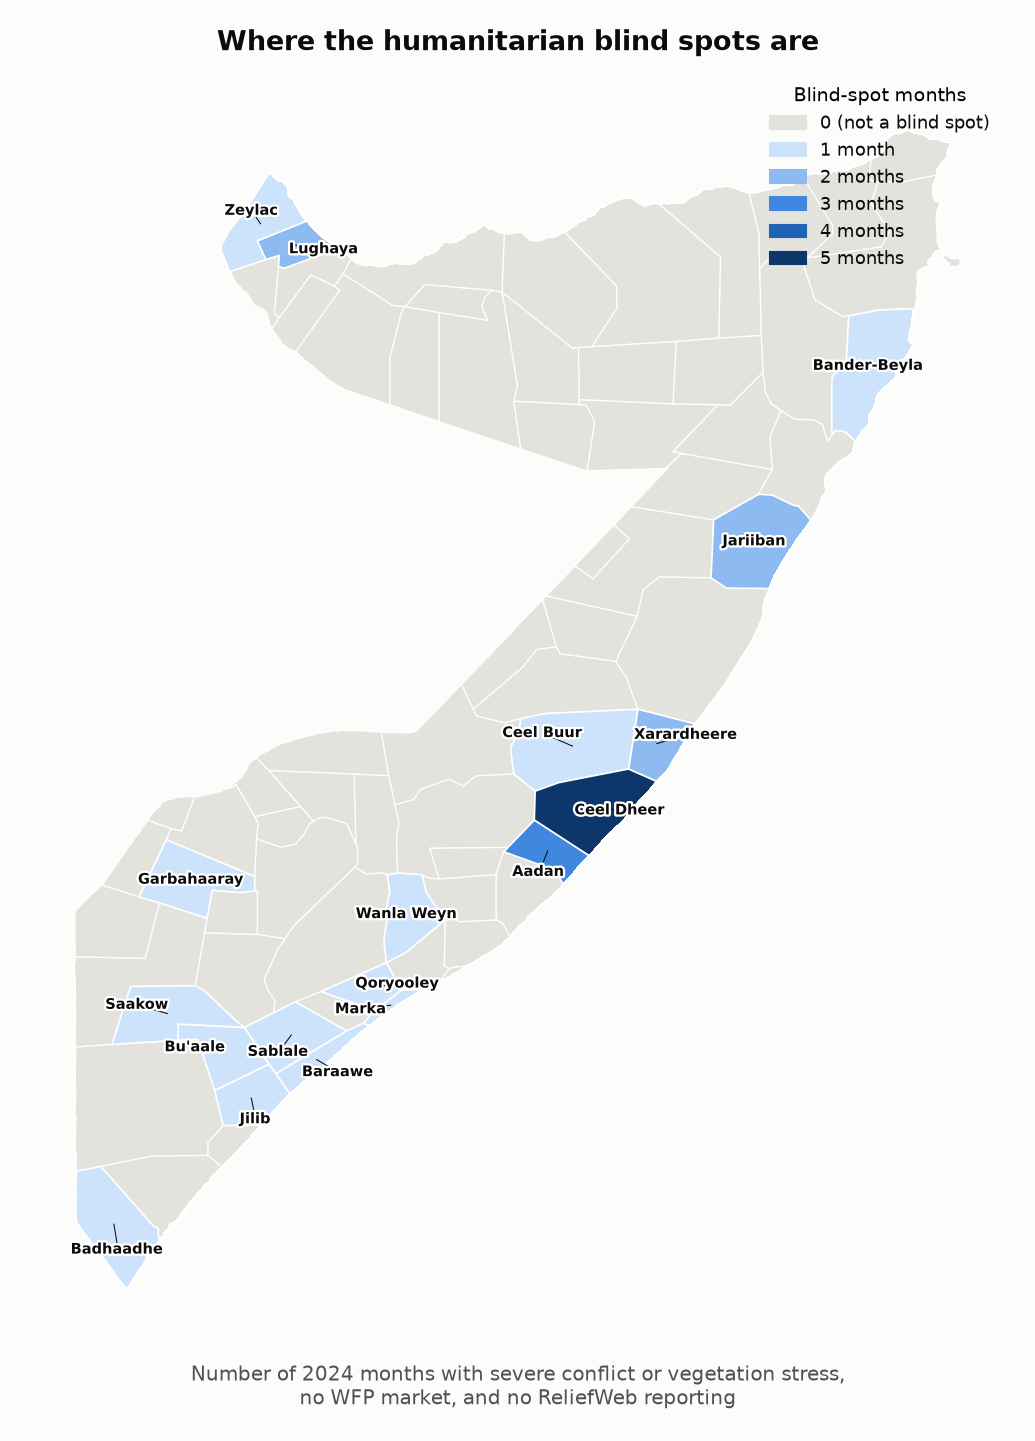
\includegraphics[width=0.62\linewidth]{blind_spots_map.png}
\caption{Number of 2024 months per district with severe conflict or vegetation stress, no WFP market, and no detected ReliefWeb district mention. Severity is defined by within-Somalia 2024 deciles, not by an external humanitarian threshold.}
\label{fig:blindspots}
\end{figure}

Overall, the Somalia analysis shows that humanitarian reporting is much more strongly associated with conflict than with vegetation stress. It also identifies district-months where severe signals were present without corresponding market or humanitarian observations. Section 4.4 considers how this finding changes when district fixed effects are introduced.

\subsection{Robustness}

Two further checks test how far the headline result from Section 4.3 can really be pushed. One of them meaningfully qualifies it. The other tests an alternative explanation without weakening it.

District fixed effects substantially qualify the interpretation of the pooled association here. The main model in Section 4.3 controls for month, but not for permanent differences between districts. Things like how accessible a district is, its population, or whether NGOs are already based there, none of that changes much from month to month. Adding a fixed effect for each district ($n = 876$, 73 districts, Banaadir excluded) removes exactly that kind of confounding. Under this stricter test, the conflict effect drops sharply. It comes out at IRR $= 1.02$ (95\% CI [0.95, 1.10], $p = 0.55$), no longer statistically significant. Vegetation stress barely moves: IRR $= 1.08$ (95\% CI [0.97, 1.20], $p = 0.16$). And the two effects are no longer significantly different from each other either (Wald chi-squared $= 0.70$, $p = 0.40$).

This does not refute Section 4.3's result; it qualifies it. A variance decomposition explains why. 70.1\% of conflict's variation happens between districts, a largely persistent property of the place, and only 29.9\% within a district over time. Vegetation stress is the mirror image: 78.9\% within, 21.1\% between. Since fixed effects use only within-district variation by design, conflict loses most of its statistical power once they are included. The most defensible reading is that the original association is largely a between-district pattern: some districts are systematically more visible than others, rather than reporting reacting to a district's own worse months.

A second check asks a different question: is the geoparser itself behind this pattern? It finds no evidence that it is. Section 3.3 noted that reports can carry geographic detail the geoparser cannot reach in the exported text. If that happened more for climate or food reports than for conflict ones, it could manufacture a false version of the Section 4.3 finding, not because conflict draws more attention but because climate-related detail is trapped more often. This was tested directly, using the same manually validated sample built for the geoparser's precision check. Two summaries of that data are available and they are not interchangeable, so both are reported. Pooling every mention together, conflict-related reports lose 84.5\% of their genuine district mentions and climate/food-related reports lose 76.8\%. Averaging within each report first, which is the unit the significance test actually compares, gives 58.2\% for conflict and 60.6\% for climate/food, running in the opposite direction. Neither comparison is statistically significant: a Mann-Whitney test on the per-report rates gives $p = 0.85$, and a Fisher's exact test on whether a report has any undetected genuine mention at all gives an odds ratio of 1.48 ($p = 0.71$). With only 16 and 17 reports in the two groups, this finds no support for the alternative explanation but is far too small to rule it out.

What this test measures should also be stated precisely. A mention is counted here when the human labeller marked a district as genuinely discussed and the geoparser did not find it in the exported title and body text. That is consistent with the detail sitting in an attachment, which is the mechanism Section 3.3 identifies, but the test does not open the attachment to confirm it; a missing alias or an unusual spelling would produce the same signature.

Together, these two checks leave Section 4.3's result standing, but bounded. The pooled association between conflict and reporting is strong and survives the topic-specific test, but the defensible reading is cross-sectional: some districts are systematically more visible than others. The stronger claim, that a district's own conflict spikes drive its own reporting spikes month to month, does not hold once permanent differences between districts are accounted for.

\clearpage
\section{Discussion, Critical Evaluation \& Recommendations}

\subsection{Limitations}

Several limitations affect how much weight the findings in Chapter 4 can bear.

The geoparser's recall is the most significant one, and the validation in Section 3.3 measures it at both levels. Precision is reasonable: roughly four in five district matches hold up under manual review, so the district matches feeding into \texttt{reports\_mentioning\_district\_count} are mostly real. Recall is where the limitation sits. The geoparser identifies that a report concerns some district 57.8\% of the time, but identifies only 17.1\% of individual report-district pairs, because the district-level detail it misses is not recoverable from the exported text alone.

This matters most for how absence is read. Every ReliefWeb-based result rests on a count that undercounts, and undercounts unevenly: a report is far more likely to be linked to one of its districts than to all of them. A district-month with zero detected mentions is therefore weaker evidence of genuine reporting absence than it appears, which is why the gaps in Section 4.3 are described as candidates rather than confirmed silences. The net direction of the bias is not knowable from these figures alone. Missed mentions inflate apparent gaps, while the roughly one in five district matches that are false positives can conceal genuine ones, so the candidate gaps reported here require case-level checking rather than being treated as either a floor or a ceiling. Neither the topic-specific test (Section 4.3) nor the attachment-bias check (Section 4.4) removes that underlying undercount.

Reading report attachments would probably help with this. ReliefWeb reports often carry an attached document, and any geographic detail held there is invisible to a geoparser that reads only the report text itself. Fetching and reading those attachments was blocked by network restrictions in the environment this dataset was built in, a real gap in what could be tested here, not something left out by choice.

There are also confounding factors this dissertation simply has no data on. Persistent NGO or humanitarian operational presence, population, road access, territorial control, any of these could independently explain why some districts are chronically more visible than others, which is exactly the kind of factor the district fixed-effects check (Section 4.4) suggests is doing real work. Without data on any of them, it's an open question whether the between-district pattern in Section 4.4 reflects genuine, self-perpetuating attention, or an unmeasured structural factor like NGO presence sitting underneath it.

The fixed-effects check itself has limited power. Each district contributes only 12 monthly observations, so a real within-district effect of moderate size could exist and still fail to reach significance. Its confidence interval (0.95 to 1.10) is consistent both with a genuinely weak effect and with one this design cannot detect from so little data per district. Section 4.4 reads best as no strong evidence of a within-district effect, rather than proof that none exists.

The attachment-content bias test in that same section rests on a small sample too, only 16 conflict-related and 17 climate/food-related reports fell cleanly into one topic group. A comparison this size has limited power to detect a real difference of moderate size. It found no evidence the geoparser favours one topic over the other, but with this few reports, that's a case of no evidence found rather than the possibility being definitively ruled out.

This dissertation is also a single-country, single-year case study. Somalia in 2024 was chosen as the empirical case through which this dissertation's methodological argument is examined. Whether the same patterns, particularly the strength of the conflict-versus-reporting relationship relative to vegetation stress, hold in other countries or years is untested here. The source-audit framework itself is meant to be reusable elsewhere, but its results in this dissertation are evidence from one case, not a general claim about humanitarian reporting behaviour.

\subsection{Implications}

The pseudo-replication error in Section 4.2 is a useful starting point. It produced a significant association that disappeared once the repeated-measures structure was accounted for, $p = 0.0001$ becoming $p = 0.18$. A researcher combining humanitarian sources without checking for this could act on a finding that does not hold. Bell et al. (2021) and Haak et al. (2018) argued in principle that integration deserves this scrutiny; this dissertation gives a concrete case of what happens without it. The source-audit framework built here, structural versus recorded availability, observed versus forecast values, and zero versus missing, is offered as a practice other humanitarian data science projects could reuse, not something specific to Somalia or to these four sources.

Committing both raw and processed data, and documenting the formula behind every engineered feature, matters for the same reason. A reader of this dissertation, or someone extending it later, can check what a ``zero'' actually means in this panel, whether a given value was observed or forecast, and exactly how a trend or standardised score was calculated. Reproducibility, in this framing, is what allows the analysis and its limitations to be independently checked by someone other than the original researcher.

The results also have something to say about prediction. Reporting attention tracks conflict far more closely than it tracks vegetation stress, and district-months exist where an extreme recorded conflict or vegetation-stress signal appeared with no WFP market observation or matched ReliefWeb report at all (Section 4.3). A prediction system trained uncritically on this kind of data could underweight climate-related food insecurity relative to conflict-related crises, reproducing the unevenness this dissertation set out to measure. This dissertation didn't train or test such a system, so this is a plausible risk raised by the findings, not a demonstrated result.

Eisensee and Str\"omberg (2007) showed that news coverage affects whether disaster relief is granted, accounting for severity. This dissertation's findings sit one step upstream: whether a crisis is reported at all, before any coverage effect on aid could begin. A district that goes structurally unreported is not just missing from the news; it may be entirely invisible to any system that treats reporting volume as a stand-in for need.

Overall, these findings suggest that data integration should be treated as part of the substantive analysis, rather than as a purely technical preprocessing step. This matters most when integrated data is later used for humanitarian monitoring or prediction, where systematic differences in reporting can become embedded directly in the resulting models.

\clearpage
\section{Conclusion \& Further Work}

This dissertation asked what methodological challenges arise when integrating heterogeneous geographic humanitarian data for crisis analysis, and how those challenges can be systematically identified. Somalia in 2024 served as the case study. Four sources, ACLED, CHIRPS and VHI, WFP, and ReliefWeb, were combined into a single Admin-2 by month dataset and audited directly rather than assumed compatible.

The sources differ substantially in spatial precision, temporal resolution, missingness, provenance and measurement uncertainty. These differences are structural properties of each source, not incidental noise. Careless integration can produce real, demonstrable failures too: a pseudo-replication error produced a statistically significant result that did not survive using the district as the unit of analysis, an unstable trend formula could have introduced invalid values silently, and a plausible-sounding engineered feature turned out to add little beyond the raw event count it was built from. Applying the source-audit framework directly to Somalia found that reporting attention tracks conflict far more strongly than it tracks vegetation stress, with 27 district-months across 18 districts where an extreme recorded conflict or vegetation-stress signal coincided with no WFP market observation and no detected ReliefWeb district mention.

The district fixed-effects check qualifies that last result. Much of the conflict-reporting association is a between-district pattern, some districts are consistently more visible than others. The evidence for a live, month-to-month reaction within a district is weak. The strongest available claim here is cross-sectional.

The main contribution of this dissertation is the source-audit framework: treating structural versus recorded availability, observed versus forecast values, and zero versus missing as distinctions worth checking explicitly, rather than assumptions to build on. Every raw and processed file behind this analysis is committed alongside the code that produced it, so the claims made here can be checked directly.

Real limits remain, and are worth restating briefly. The geoparser bounds every ReliefWeb-based result: precision is reasonable at roughly 80\%, but pair-level recall of 17.1\% means the reporting counts undercount, and a district-month with no detected mention is weak evidence that nothing was published. Several plausible confounders, NGO presence, population, road access, territorial control, could not be tested with the data available. This is one country, one year; whether the same pattern holds elsewhere is untested.

The natural next steps follow from these limits: comparing this dataset's own severity assessment against an external benchmark, testing whether slow-onset crises are reported late rather than never, and extending the same source-audit approach to other countries WFP tracks. Combining humanitarian data sources is a decision with consequences for what a study can conclude, not a neutral technical step, and this dissertation is one demonstration of what happens when that decision gets examined rather than assumed.

% =====================================================================
% REFERENCES (manually formatted Harvard style, plain text -- no BibTeX
% needed since in-text citations above are already typed as plain text)
% =====================================================================
\begingroup
\clearpage
\section*{References Cited}
\addcontentsline{toc}{section}{References Cited}
\begin{list}{}{\setlength{\leftmargin}{1cm}\setlength{\itemindent}{-1cm}\setlength{\itemsep}{8pt}}

\item Bell, D., Lycett, M., Marshan, A. and Monaghan, A. (2021) `Exploring future challenges for big data in the humanitarian domain', \textit{Journal of Business Research}, 131, pp. 453--468.

\item Centre for Humanitarian Data (no date) \textit{What are the HDX Data Grids?} Available at: \url{https://centre.humdata.org/ufaqs/what-is-the-data-criteria-for-the-data-grids/} (Accessed: 12 September 2026).

\item Eisensee, T. and Str\"omberg, D. (2007) `News droughts, news floods, and U.S. disaster relief', \textit{The Quarterly Journal of Economics}, 122(2), pp. 693--728.

\item Food Security and Nutrition Analysis Unit (FSNAU) (no date) \textit{Markets}. Available at: \url{http://fsnau.org/sectors/markets} (Accessed: 12 September 2026).

\item Funk, C., Peterson, P., Landsfeld, M., Pedreros, D., Verdin, J., Shukla, S., Husak, G., Rowland, J., Harrison, L., Hoell, A. and Michaelsen, J. (2015) `The climate hazards infrared precipitation with stations, a new environmental record for monitoring extremes', \textit{Scientific Data}, 2, article 150066.

\item GADM (2022) \textit{GADM database of Global Administrative Areas, version 4.1}. Available at: \url{https://gadm.org} (Accessed: 12 September 2026).

\item Haak, E., Ubacht, J., Van den Homberg, M., Cunningham, S. and Van de Walle, B. (2018) `A framework for strengthening data ecosystems to serve humanitarian purposes', in \textit{Proceedings of the 19th Annual International Conference on Digital Government Research (dg.o '18)}. New York: Association for Computing Machinery.

\item Hendrix, C.S. (2017) `The streetlight effect in climate change research on Africa', \textit{Global Environmental Change}, 43, pp. 137--147.

\item Marshak, A., Young, H. and Naumova, E.N. (2023) `Data on humanitarian crises: who and what are we missing?', \textit{Food and Nutrition Bulletin}, 44(2) (supplement), pp. S124--S126.

\item Miller, E., Kishi, R., Raleigh, C. and Dowd, C. (2022) `An agenda for addressing bias in conflict data', \textit{Scientific Data}, 9, article 593.

\item NOAA/NESDIS Center for Satellite Applications and Research (STAR) (no date) \textit{Global Vegetation Health Products}. Available at: \url{https://www.star.nesdis.noaa.gov/smcd/emb/vci/VH/} (Accessed: 12 September 2026).

\item Raleigh, C., Linke, A., Hegre, H. and Karlsen, J. (2010) `Introducing ACLED: an armed conflict location and event dataset', \textit{Journal of Peace Research}, 47(5), pp. 651--660.

\item ReliefWeb (no date) \textit{Review and redesign of the minimum expenditure basket in Somalia: the Basic MEB and the Sector Standard MEB}. Available at: \url{https://reliefweb.int/report/somalia/review-and-redesign-minimum-expenditure-basket-somalia-basic-meb-and-sector-standard-meb} (Accessed: 12 September 2026).

\item UN Office for the Coordination of Humanitarian Affairs (OCHA) (no date) \textit{ReliefWeb}. Available at: \url{https://reliefweb.int} (Accessed: 12 September 2026).

\item Weidmann, N.B. (2016) `A closer look at reporting bias in conflict event data', \textit{American Journal of Political Science}, 60(1), pp. 206--218.

\item World Food Programme (2014) \textit{Technical guidance note: calculation and use of the Alert for Price Spikes (ALPS) indicator}. Available at: \url{https://reliefweb.int/report/world/technical-guidance-note-calculation-and-use-alert-price-spikes-alps-indicator-april} (Accessed: 12 September 2026).

\item World Food Programme (no date) \textit{VAM Economic Explorer: food prices}. Available at: \url{https://dataviz.vam.wfp.org/economic_explorer/prices} (Accessed: 12 September 2026).

\end{list}
\endgroup

% =====================================================================
% APPENDICES
% =====================================================================
\appendix
\clearpage
\section*{Appendices}
\addcontentsline{toc}{section}{Appendices}

\subsection*{Appendix A: Engineered Feature Reference}
\addcontentsline{toc}{subsection}{Appendix A: Engineered Feature Reference}

The committed dataset contains 25 columns in total: 5 identifiers (\texttt{location\_id}, \texttt{country\_code}, \texttt{admin1}, \texttt{admin2}, \texttt{time\_id}), 1 structural flag (\texttt{has\_market\_coverage}), and the 19 engineered features listed below. The table also lists four further variables (\texttt{log\_conflict}, \texttt{vegetation\_stress}, \texttt{conflict\_z}, \texttt{vhi\_stress\_z}) that are computed only at modelling time from the 19 and are not stored in the committed panel itself.

\footnotesize
\begin{longtable}{p{4cm}p{4.3cm}p{5.7cm}}
\toprule
\textbf{Feature} & \textbf{Description} & \textbf{Formula} \\
\midrule
\endfirsthead
\toprule
\textbf{Feature} & \textbf{Description} & \textbf{Formula} \\
\midrule
\endhead
\texttt{location\_id} & District identifier & Identifier, not computed \\
\texttt{country\_code} & Country identifier (Somalia) & Identifier, not computed \\
\texttt{admin1} & Region name & Identifier, not computed \\
\texttt{admin2} & District name & Identifier, not computed \\
\texttt{time\_id} & Year-month identifier & Identifier, not computed \\
\texttt{has\_market\_coverage} & Whether WFP monitors any market in this district, in any month of 2024 & Structural flag, fixed for the whole year \\
\texttt{conflict\_event\_count} & Number of ACLED conflict events & COUNT(events), grouped by district and month \\
\texttt{fatalities} & Total conflict deaths reported & SUM(fatalities), grouped by district and month \\
\texttt{conflict\_trend\_log} & Month-over-month change in conflict activity & $\ln(1+\text{count}_t) - \ln(1+\text{count}_{t-1})$ \\
\texttt{rainfall\_mean\_mm} & Average monthly rainfall & zonal\_mean$(D)$ over the CHIRPS raster for the month \\
\texttt{vegetation\-\_health\-\_index\-\_mean} & Average vegetation health, used as a drought proxy & Day-weighted mean of weekly VHI zonal means overlapping the month \\
\texttt{*\_price\_usd} (wheatflour / rice / sugar / oil) & Commodity price converted to USD & price\_local / exchange\_rate\_to\_usd \\
\texttt{*\_trend\_log} (wheatflour / rice / sugar / oil) & Month-over-month price change per commodity & $\ln(\text{price}_t) - \ln(\text{price}_{t-1})$ \\
\texttt{*\_pewi\_score} (wheatflour / rice / sugar / oil) & WFP's Price Early Warning Indicator per commodity & $(P_t - \hat{P}_t)/\sigma_\varepsilon$; taken directly from WFP, not recomputed \\
\texttt{reports\-\_mentioning\-\_district\-\_count} & ReliefWeb reports referencing this district that month & COUNT of reports matching the district's name or a documented alias \\
\texttt{food\-\_nutrition\-\_report\-\_count} & Same, restricted to reports tagged Food and Nutrition & COUNT of matched reports where themes contains ``Food and Nutrition'' \\
\midrule
\multicolumn{3}{l}{\textit{Modelling-only, not stored in the committed panel:}} \\
\texttt{log\_conflict} & Logged conflict count, used only for modelling & $\ln(1+\text{conflict\_event\_count})$ \\
\texttt{vegetation\_stress} & Vegetation stress, sign-flipped so higher always means worse & $-\text{vegetation\_health\_index\_mean}$ \\
\texttt{conflict\_z} & Standardised logged conflict, used in regression models & $(\text{log\_conflict} - \bar{x})/s$ \\
\texttt{vhi\_stress\_z} & Standardised vegetation stress, used in regression models & $(\text{vegetation\_stress} - \bar{x})/s$ \\
\bottomrule
\caption{Complete engineered feature reference.} \label{tab:appA} \\
\end{longtable}

\subsection*{Appendix B: Source-Quality Table}
\addcontentsline{toc}{subsection}{Appendix B: Source-Quality Table}

The table below summarises how the four data sources differ across seven dimensions: native spatial and temporal granularity, collection mechanism, structural availability, recorded coverage, what a zero means, what missing means, and the main measurement limitation of each source.

\begingroup
\footnotesize
\begin{longtable}{p{2.0cm}p{2.95cm}p{2.95cm}p{2.95cm}p{2.95cm}}
\toprule
\textbf{Dimension} & \textbf{Conflict (ACLED)} & \textbf{Climate (CHIRPS/VHI)} & \textbf{Market (WFP/PEWI)} & \textbf{Reporting (ReliefWeb)} \\
\midrule
\endfirsthead
\toprule
\textbf{Dimension} & \textbf{Conflict (ACLED)} & \textbf{Climate (CHIRPS/VHI)} & \textbf{Market (WFP/PEWI)} & \textbf{Reporting (ReliefWeb)} \\
\midrule
\endhead
Native spatial granularity & Event-level, geocoded, but 77.5\% exact site, 22.4\% approximate, 0.1\% broad area only & Satellite grid cells: CHIRPS 0.05 degrees, VHI 0.036 degrees & A specific, named market within a district & A whole document; never more precise than ``mentions this district'' \\
Native temporal granularity & Daily events, aggregated to month & CHIRPS monthly; VHI weekly, day-weighted to month & Enumerator visits, roughly weekly, aggregated monthly & Report publish date; no fixed schedule \\
Collection mechanism & Media and monitoring-partner coding (65.3\% cite a local partner) & Satellite imagery, algorithmic, no ground survey required & Weekly market surveys by WFP enumerators & Reports published by humanitarian organisations, curated and tagged \\
Structural availability & All 74 districts & All 74 districts, uniformly & 35 of 74 districts (47.3\%) only & In principle any of 74, limited by attention and geoparsing \\
Recorded coverage & 100\% (zero-filled by construction) & 100\%, never missing & 47.2\% by price, 43.1\% by PEWI & 60.1\% of district-months have $\geq 1$ report \\
What a zero means & Genuine calm or unreported violence, indistinguishable & A real, meaningful low reading & Not valid for price itself; only derived counts can be 0 & No exported text matched; may be an unread attachment \\
What missing means & Does not occur (zero-filled) & Does not occur in this panel & No monitored market, or a genuine data gap & Does not occur as distinct from zero \\
\bottomrule
\caption{Source-quality comparison across all four sources.} \label{tab:appB} \\
\end{longtable}
\endgroup

\subsection*{Appendix C: Month-by-Month Source Coverage}
\addcontentsline{toc}{subsection}{Appendix C: Month-by-Month Source Coverage}

The table below shows, for each month of 2024, the percentage (and count) of the 74 districts covered by each of the four sources. ``Covered'' is defined at the district-month level: at least one conflict event for Conflict, both a rainfall and vegetation reading for Climate, at least one price or PEWI value for Market, and at least one matched report for Reporting.

\begin{longtable}{lcccc}
\toprule
\textbf{Month} & \textbf{Conflict} & \textbf{Climate} & \textbf{Market} & \textbf{Reporting} \\
\midrule
\endfirsthead
\toprule
\textbf{Month} & \textbf{Conflict} & \textbf{Climate} & \textbf{Market} & \textbf{Reporting} \\
\midrule
\endhead
January & 66.2\% (49/74) & 100.0\% (74/74) & 45.9\% (34/74) & 51.4\% (38/74) \\
February & 59.5\% (44/74) & 100.0\% (74/74) & 47.3\% (35/74) & 50.0\% (37/74) \\
March & 56.8\% (42/74) & 100.0\% (74/74) & 47.3\% (35/74) & 60.8\% (45/74) \\
April & 50.0\% (37/74) & 100.0\% (74/74) & 47.3\% (35/74) & 67.6\% (50/74) \\
May & 59.5\% (44/74) & 100.0\% (74/74) & 47.3\% (35/74) & 64.9\% (48/74) \\
June & 62.2\% (46/74) & 100.0\% (74/74) & 47.3\% (35/74) & 56.8\% (42/74) \\
July & 59.5\% (44/74) & 100.0\% (74/74) & 47.3\% (35/74) & 66.2\% (49/74) \\
August & 59.5\% (44/74) & 100.0\% (74/74) & 47.3\% (35/74) & 50.0\% (37/74) \\
September & 68.9\% (51/74) & 100.0\% (74/74) & 47.3\% (35/74) & 45.9\% (34/74) \\
October & 63.5\% (47/74) & 100.0\% (74/74) & 47.3\% (35/74) & 66.2\% (49/74) \\
November & 58.1\% (43/74) & 100.0\% (74/74) & 47.3\% (35/74) & 73.0\% (54/74) \\
December & 58.1\% (43/74) & 100.0\% (74/74) & 47.3\% (35/74) & 68.9\% (51/74) \\
\bottomrule
\caption{Percentage of the 74 districts covered by each source, month by month (2024).} \label{tab:appC} \\
\end{longtable}

\noindent Climate is the only source that never moves, sitting at 100\% every month because satellite coverage is unconditional. Market barely moves either, 34 or 35 districts in every single month. Conflict and Reporting are the two sources that genuinely fluctuate: Conflict ranges from 37 to 51 districts (50.0\% to 68.9\%), and Reporting swings the widest of all four, from 34 to 54 districts (45.9\% to 73.0\%).

\subsection*{Appendix D: Logistic Regression Model Diagnostics}
\addcontentsline{toc}{subsection}{Appendix D: Logistic Regression Model Diagnostics}

The table below reports full in-sample and out-of-sample diagnostics for the logistic regression predicting whether a district is mentioned that month (Section 3.5), for both the full model (conflict, market, climate, region and month) and a parsimonious model (conflict, market and month, with region and climate removed). Out-of-sample figures use 5-fold group cross-validation holding out whole districts.

\begin{table}[h!]
\centering
\begin{tabular}{lcc}
\toprule
\textbf{Metric} & \textbf{In-sample} & \textbf{Out-of-sample} \\
\midrule
AUC & 0.776 & 0.641 \\
Accuracy & 0.723 & 0.638 \\
Precision (of predicted yes) & 0.743 & 0.685 \\
Recall / sensitivity & 0.816 & 0.726 \\
Specificity & 0.585 & 0.508 \\
F1 & 0.778 & 0.705 \\
Brier score (lower = better) & 0.186 & 0.240 \\
McFadden pseudo R\textsuperscript{2} & 0.184 & --- \\
\bottomrule
\end{tabular}
\caption{Full model diagnostics.}
\end{table}

\noindent Out-of-sample confusion matrix (full model): of district-months truly not mentioned, 180 were correctly predicted no and 174 incorrectly predicted yes; of district-months truly mentioned, 143 were incorrectly predicted no and 379 correctly predicted yes.

\begin{table}[h!]
\centering
\begin{tabular}{lcc}
\toprule
\textbf{Metric} & \textbf{In-sample} & \textbf{Out-of-sample} \\
\midrule
AUC & 0.739 & 0.716 \\
Accuracy & 0.684 & 0.663 \\
Precision (of predicted yes) & 0.716 & 0.699 \\
Recall / sensitivity & 0.778 & 0.762 \\
Specificity & 0.545 & 0.517 \\
F1 & 0.746 & 0.730 \\
Brier score (lower = better) & 0.201 & 0.211 \\
McFadden pseudo R\textsuperscript{2} & 0.133 & --- \\
\bottomrule
\end{tabular}
\caption{Parsimonious model diagnostics (region and climate removed).}
\end{table}

\noindent Out-of-sample confusion matrix (parsimonious model): of district-months truly not mentioned, 183 were correctly predicted no and 171 incorrectly predicted yes; of district-months truly mentioned, 124 were incorrectly predicted no and 398 correctly predicted yes.

\textit{The parsimonious model, without region or climate, generalises better out-of-sample (AUC 0.716 versus 0.641) despite a lower in-sample AUC, which is why Section 3.5 and Section 4 treat region's apparent explanatory power with caution.}

\subsection*{Appendix E: Regression Model Specifications}
\addcontentsline{toc}{subsection}{Appendix E: Regression Model Specifications}

This appendix sets out the exact specification of every regression used in Chapter 4, referenced from section 3.5.

\begingroup
\setlength{\intextsep}{0pt}
\setlength{\floatsep}{0pt}
\setlength{\textfloatsep}{0pt}
\setlength{\abovecaptionskip}{6pt}
\setlength{\belowcaptionskip}{6pt}
\begin{table}[h!]
\centering
\begin{tabular}{p{2.9cm}p{2.7cm}p{4.3cm}p{1.4cm}p{2.5cm}}
\toprule
\textbf{Model} & \textbf{Outcome} & \textbf{Predictors} & \textbf{Fixed effects} & \textbf{Standard errors} \\
\midrule
Main NB (Section 4.3) & Reports mentioning district & conflict\_z, vhi\_stress\_z, month & None & Clustered by district \\
Food/Nutrition NB (Section 4.3) & Food/nutrition reports & conflict\_z, vhi\_stress\_z, month & None & Clustered by district \\
Fixed-effects NB (Section 4.4) & Reports mentioning district & conflict\_z, vhi\_stress\_z, month & District & Clustered by district \\
Logistic (Section 3.5) & Mentioned (yes/no) & conflict, market presence, rainfall, vegetation stress, region, month & None & Clustered by district \\
\bottomrule
\end{tabular}
\caption{Regression specifications used in Chapter 4.}
\label{tab:modelspecs}
\end{table}
\endgroup

\subsection*{Appendix F: Project Proposal and Ethics Screening Form}
\addcontentsline{toc}{subsection}{Appendix F: Project Proposal and Ethics Screening Form}

\noindent\includegraphics[width=15.9cm,height=7.13cm]{proposal_form_logo.jpg}

\vspace{8pt}
\noindent\textbf{CST4990 - Dissertation Proposal Form}

\noindent Date of Submission: 29/05/2026

\vspace{8pt}
\begingroup
\renewcommand{\arraystretch}{1.2}
\setlength{\intextsep}{0pt}
\setlength{\floatsep}{0pt}
\setlength{\textfloatsep}{0pt}
\setlength{\abovecaptionskip}{6pt}
\setlength{\belowcaptionskip}{6pt}
\begin{table}[h!]
\centering
\begin{tabular}{|p{4cm}|p{10.7cm}|}
\hline
\textbf{Name} & Samuel Aracena \\
\hline
\textbf{Student Id} & M01078358 \\
\hline
\textbf{Programme of Study} & MSc Data Science \\
\hline
\textbf{Project Title} & Integrating heterogeneous humanitarian data for crisis analysis: a source-audit framework applied to Somalia \\
\hline
\textbf{Campus} & HEN $\boxtimes$ \qquad MRU $\Box$ \qquad DBI $\Box$ \\
\hline
\textbf{Supervisor Name} & Giovanni Quattrone \\
\hline
\textbf{Supervisor Approval} & Yes $\boxtimes$ \qquad\qquad No $\Box$ \\
\hline
\textbf{Supervisor Signature} & \\
\hline
\end{tabular}
\caption{Project Proposal Form: submission and applicant details.}
\end{table}
\endgroup

\vspace{10pt}
\noindent\textbf{Section 1: Academic}

\noindent This section helps academic staff evaluate your project's viability and assign a suitable supervisor. It will also serve as a basis for workshop discussions with your supervisor.

\vspace{8pt}
\begingroup
\footnotesize
\noindent\textbf{Table: Project Proposal Form, Section 1 Academic.}

\vspace{4pt}
\noindent\fbox{\begin{minipage}{\dimexpr\linewidth-2\fboxsep-2\fboxrule\relax}
\textbf{STUDENT NAME:} Samuel Aracena
\end{minipage}}

\noindent\fbox{\begin{minipage}{\dimexpr\linewidth-2\fboxsep-2\fboxrule\relax}
\textbf{STUDENT NUMBER:} M01078358
\end{minipage}}

\noindent\fbox{\begin{minipage}{\dimexpr\linewidth-2\fboxsep-2\fboxrule\relax}
\textbf{PROPOSED TITLE OF PROJECT:} Integrating heterogeneous humanitarian data for crisis analysis: a source-audit framework applied to Somalia
\end{minipage}}

\noindent\fbox{\begin{minipage}{\dimexpr\linewidth-2\fboxsep-2\fboxrule\relax}
\textbf{BRIEFLY DISCUSS THE PROBLEM THAT YOU ARE INVESTIGATING AND CITE RELEVANT REFERENCES. (max 300 words)}

Humanitarian crisis analysis increasingly relies on combining heterogeneous geographic data sources such as conflict-event databases, satellite observations, market-monitoring systems and humanitarian reports. These sources are often treated as compatible inputs to downstream models, while the integration process itself is considered a technical preprocessing step.

This study starts from a different position: data integration is itself a methodological problem that can materially affect scientific conclusions.

The sources used here differ in how they observe reality, at what spatial and temporal resolution they operate, how missing values arise, how locations are represented, and whether observations are genuinely measured or model-generated. The Somalia case study shows that these differences are not minor implementation details. They can affect coverage estimates, engineered features, statistical significance and the apparent relationship between crisis signals and humanitarian attention.
\end{minipage}}

\noindent\fbox{\begin{minipage}{\dimexpr\linewidth-2\fboxsep-2\fboxrule\relax}
\textbf{GIVE YOUR RESEARCH QUESTIONS (Max 3) AND/OR AIMS \& OBJECTIVES}

RQ1. Data integration and quality: How do humanitarian sources differ in spatial granularity, temporal resolution, missingness, provenance and measurement uncertainty?

RQ2. Failure modes: Which integration choices can introduce misleading coverage estimates, invalid features or incorrect statistical conclusions?

RQ3. Empirical consequences: What does applying a source-aware integration framework to Somalia reveal about humanitarian observability and reporting bias?
\end{minipage}}

\noindent\fbox{\begin{minipage}{\dimexpr\linewidth-2\fboxsep-2\fboxrule\relax}
\textbf{IDENTIFY YOUR RESEARCH METHODS} (e.g. Data collection methods such as surveys, interviews, Data Analysis - qualitative and/or qualitative; Product development methods)

Data will be preprocessed and analysed using Python. Various Python libraries, machine learning techniques, and NLP methods will be explored throughout the project
\end{minipage}}

\noindent\fbox{\begin{minipage}{\dimexpr\linewidth-2\fboxsep-2\fboxrule\relax}
\textbf{WHAT ARE THE PROBABLE PROJECT OUTCOMES?} (E.g. recommendations, a new model or framework, new software etc)

This dissertation's main outcome is a source-audit framework for combining heterogeneous humanitarian data, checking each source for structural versus recorded availability, observed versus forecast values, and zero versus missing. Applied to a Somalia 2024 case study, it catches real integration failures (including a false-positive result caused by treating repeated observations as independent) and shows that humanitarian reporting tracks conflict far more strongly than it tracks vegetation stress, with district-months where a severe crisis existed and no data was recorded at all. The core contribution is methodological: demonstrating that combining humanitarian data sources is a consequential decision, not a neutral technical step.
\end{minipage}}

\noindent\fbox{\begin{minipage}{\dimexpr\linewidth-2\fboxsep-2\fboxrule\relax}
\textbf{IDENTIFY ANY TECHNICAL RESOURCES NEEDED} (e.g. Hardware, software)

Project will be completed in a Python notebook environment using a computer.
\end{minipage}}

\noindent\fbox{\begin{minipage}{\dimexpr\linewidth-2\fboxsep-2\fboxrule\relax}
\textbf{IDENTIFY ANY POSSIBLE CONSTRAINTS} (This includes any problems you may encounter with resources or other things necessary to carry out your study)

One limitation of this study is that humanitarian news datasets may contain missing events, inaccurate locations, duplicate reports, or uneven reporting coverage across regions and time periods. Differences in event coding systems between GDELT, ReliefWeb, and ICEWS may also make direct comparison difficult.

From an ethical perspective, the project uses publicly available datasets and does not involve human participants. However, humanitarian news reporting may contain reporting bias or underrepresent certain regions and populations. The study will therefore consider issues related to data quality, observability bias, and responsible use of humanitarian data
\end{minipage}}

\noindent\fbox{\begin{minipage}{\dimexpr\linewidth-2\fboxsep-2\fboxrule\relax}
\textbf{GIVE A PROJECT SCHEDULE} (Proposed progress by each week until submission date.)

The proposed project will follow the schedule below:
\begin{itemize}[leftmargin=1.2em,itemsep=0pt,topsep=2pt]
\item Weeks 1--2: Literature review and data familiarisation
\item Weeks 3--4: Data preprocessing and exploratory analysis
\item Weeks 5--7: Method development and modelling
\item Weeks 8--9: Evaluation and visualisation
\item Week 10: Final write-up and presentation preparation
\end{itemize}
\end{minipage}}

\noindent\fbox{\begin{minipage}{\dimexpr\linewidth-2\fboxsep-2\fboxrule\relax}
(staff use only) Project Approved by Academic Team? Please tick \quad YES $\Box$ \quad NO $\Box$
\end{minipage}}

\noindent\fbox{\begin{minipage}{\dimexpr\linewidth-2\fboxsep-2\fboxrule\relax}
Academic Staff comments:
\end{minipage}}
\endgroup

\vspace{10pt}
\noindent\textbf{Section 2: Ethics Review and Approval}

\noindent This Research Ethics Screening Form will enable taught students to self-assess and determine whether their research requires ethical review and approval via the online Ethics Monitor before commencing their study. Supervisors must approve this form after consultation with students.

\vspace{4pt}
\noindent M - Minimal Risk; \quad X - More than Minimal Risk. \quad H - High Risk

\vspace{8pt}
\begingroup
\footnotesize
\begin{longtable}{|p{10.3cm}|p{1.4cm}|p{1.4cm}|}
\hline
\textbf{Please answer whether your research/study involves any of the following:} & & \\
\hline
\endfirsthead
\hline
\textbf{Please answer whether your research/study involves any of the following:} & & \\
\hline
\endhead
{\ttfamily o}\quad \textsuperscript{H}ANIMALS or animal parts. & $\Box$ Yes & $\boxtimes$ No \\ \hline
{\ttfamily o}\quad \textsuperscript{M}CELL LINES (established and commercially available cells, biological research). & $\Box$ Yes & $\boxtimes$ No \\ \hline
{\ttfamily o}\quad \textsuperscript{H}CELL CULTURE (Primary: from animal/human cells, biological research). & $\Box$ Yes & $\boxtimes$ No \\ \hline
{\ttfamily o}\quad \textsuperscript{H}CLINICAL Audits or Assessments (e.g.\ in medical settings). & $\Box$ Yes & $\boxtimes$ No \\ \hline
{\ttfamily o}\quad \textsuperscript{X}CONFLICT of INTEREST or lack of IMPARTIALITY. If unsure see ``Code of Practice for Research'' (Sec 3.5) at: \url{https://unihub.mdx.ac.uk/study/spotlights/types/research-at-middlesex/research-ethics} & $\Box$ Yes & $\boxtimes$ No \\ \hline
{\ttfamily o}\quad \textsuperscript{X}DATA to be used that is not freely available (e.g. secondary data needing permission for access or use). & $\Box$ Yes & $\boxtimes$ No \\ \hline
{\ttfamily o}\quad \textsuperscript{X}DAMAGE (e.g., to precious artefacts or to the environment) or present a significant risk to society). & $\Box$ Yes & $\boxtimes$ No \\ \hline
{\ttfamily o}\quad \textsuperscript{X}EXTERNAL ORGANISATION, research carried out within an external organisation or your research is commissioned by a government (or government body). & $\Box$ Yes & $\boxtimes$ No \\ \hline
{\ttfamily o}\quad \textsuperscript{M}FIELDWORK (e.g., biological research, ethnography studies). & $\Box$ Yes & $\boxtimes$ No \\ \hline
{\ttfamily o}\quad \textsuperscript{H}GENETICALLTY MODIFIED ORGANISMS (GMOs) (biological research). & $\Box$ Yes & $\boxtimes$ No \\ \hline
{\ttfamily o}\quad \textsuperscript{H}GENE THERAPY including DNA sequenced data (biological research). & $\Box$ Yes & $\boxtimes$ No \\ \hline
{\ttfamily o}\quad \textsuperscript{M}HUMAN PARTICIPANTS, ANONYMOUS Questionnaires (participants not identified or identifiable). & $\Box$ Yes & $\boxtimes$ No \\ \hline
{\ttfamily o}\quad \textsuperscript{X}HUMAN PARTICIPANTS, IDENTIFIABLE (participants are identified or can be identified): survey questionnaire/ INTERVIEWS / focus groups / experiments / observation studies/ evaluation studies. & $\Box$ Yes & $\boxtimes$ No \\ \hline
{\ttfamily o}\quad \textsuperscript{H}HUMAN TISSUE (e.g., human relevant material, e.g., blood, saliva, urine, breast milk, faecal material). & $\Box$ Yes & $\boxtimes$ No \\ \hline
{\ttfamily o}\quad \textsuperscript{H}ILLEGAL/HARMFUL activities research (e.g., development of technology intended to be used in an illegal/harmful context or to breach security systems, searching the internet for information on highly sensitive topics such as child and extreme pornography, terrorism, use of the DARK WEB, research harmful to national security). & $\Box$ Yes & $\boxtimes$ No \\ \hline
{\ttfamily o}\quad \textsuperscript{X}PERMISSION is required to access premises or research participants. & $\Box$ Yes & $\boxtimes$ No \\ \hline
{\ttfamily o}\quad \textsuperscript{X}PERSONAL DATA PROCESSING (Any activity with data that can directly or indirectly identify a living person). For example, data gathered from interviews, databases, digital devices such as mobile phones, social media or internet platforms or apps with or without individuals'/owners' knowledge or consent, and/or could lead to individuals/owners being IDENTIFIED or SPECIAL CATEGORY DATA (GDPR\textsuperscript{1}) or CRIMINAL OFFENCE DATA. \textsuperscript{1}Special category data (GDPR, Art.9): ``personal data revealing racial or ethnic origin, political opinions, religious or philosophical beliefs, or trade union membership, and the processing of genetic data, biometric data for the purpose of uniquely identifying a natural person, data concerning health or data concerning a natural person's sex life or sexual orientation''. & $\Box$ Yes & $\boxtimes$ No \\ \hline
{\ttfamily o}\quad \textsuperscript{X}PUBLIC WORKS DOCTORATES: Evidence of permission is required for use of works/artifacts (that are protected by Intellectual Property (IP) Rights, e.g. copyright, design right) in a doctoral critical commentary when the IP in the work/artifacts jointly prepared/produced or is owned by another body & $\Box$ Yes & $\boxtimes$ No \\ \hline
{\ttfamily o}\quad \textsuperscript{H}RISK OF PHYSICAL OR PSYCHOLOGICAL HARM (e.g., TRAVEL to dangerous places in your own country or in a foreign country, research with NGOs/humanitarian groups in conflict/dangerous zones, development of technology/agent/chemical that may be harmful to others, any other foreseeable dangerous risks). & $\Box$ Yes & $\boxtimes$ No \\ \hline
{\ttfamily o}\quad \textsuperscript{X}SECURITY CLEARANCE, required for research. & $\Box$ Yes & $\boxtimes$ No \\ \hline
{\ttfamily o}\quad \textsuperscript{X}SENSITIVE TOPICS (e.g., anything deeply personal and distressing, taboo, intrusive, stigmatising, sexual in nature, potentially dangerous, etc). & $\Box$ Yes & $\boxtimes$ No \\ \hline
\hline
\caption{Research Ethics Screening Form.} \label{tab:ethicsform} \\
\end{longtable}
\endgroup

\vspace{4pt}
\noindent If you have answered `Yes' to ANY of the items in the table, your application REQUIRES ethical review and approval using the online Ethics Monitor BEFORE commencing your research. Please apply for ethical review and approval using the Ethics Monitor. Further information such as links to Ethics Monitor and training videos is available at MyLearning (Middlesex Online Research Ethics) area: \url{https://mdx.mrooms.net/course/view.php?id=12277} (Login required).

\vspace{4pt}
\noindent If you have answered `No' to ALL of the items in the table, your application is Low Risk and you may NOT require ethical review and approval using Ethics Monitor before commencing your research. Your research supervisor will confirm this below.

\vspace{10pt}
\noindent Student Signature: \textit{Samuel Aracena} \qquad Date: 29/05/2026

\vspace{8pt}
\noindent\textbf{To be completed by the supervisor:}

\vspace{6pt}
\begingroup
\renewcommand{\arraystretch}{1.3}
\setlength{\intextsep}{0pt}
\setlength{\floatsep}{0pt}
\setlength{\textfloatsep}{0pt}
\setlength{\abovecaptionskip}{6pt}
\setlength{\belowcaptionskip}{6pt}
\begin{table}[h!]
\centering
\begin{tabular}{|p{10.5cm}|p{2.5cm}|}
\hline
\textbf{Based on the details provided in the self-assessment form, I confirm that:} & \textbf{Insert Y or N} \\
\hline
The study is Low Risk and does not require ethical review \& approval using Ethics Monitor & \\
\hline
The study requires ethical review and approval using Ethics Monitor. & \\
\hline
\end{tabular}
\caption{Supervisor confirmation and risk determination.}
\end{table}
\endgroup

\vspace{10pt}
\noindent Supervisor Signature: \rule{6cm}{0.4pt} \qquad Date: \rule{3cm}{0.4pt}

\end{document}
